% Method section for the Introspective Verification paper.
% Style: plain, direct; no em-dashes; minimal colons/quotes; no anthropomorphic verbs.

\section{Method}
\label{sec:method}

We describe the introspective verdict head, which reads a per step reward from the backbone's hidden states in a single forward pass. We fix notation (\Cref{sec:method-setup}), define the head (\Cref{sec:method-head}), explain the layer choice (\Cref{sec:method-layer}), state the training objective (\Cref{sec:method-train}), and give the inference procedure and its cost (\Cref{sec:method-infer}). An optional logit space fusion with a generative verifier is in \Cref{sec:method-fusion}.

\subsection{Setup and notation}
\label{sec:method-setup}

A problem $x$ has a candidate solution written as an ordered sequence of steps $s_1,\dots,s_k$. A process verifier assigns each step a reward $r_i \in [0,1]$, where a reward above a threshold marks the step as an error, and the first such step is the located error. ProcessBench scores this located first error against the labeled one.

The backbone is a decoder only transformer $f$ with $L$ layers. For an input token sequence it returns hidden states $h^{(0)},\dots,h^{(L)}$, where $h^{(0)}$ is the embedding and $h^{(L)}$ is the final layer. We write $h_i^{(\ell)} \in \R^{d}$ for the hidden state at layer $\ell$ at the last token of step $s_i$, that is the token that ends the step in the concatenation $x, s_1, \dots, s_k$. Because attention is causal, this last token has attended to all of $x$ and $s_1,\dots,s_i$, so its hidden state is a natural summary of the step in the context that precedes it. Reading a per step reward from $h_i^{(\ell)}$ therefore requires no extra generation, only the states that a single pass over the solution already produces.

\subsection{The introspective verdict head}
\label{sec:method-head}

The head sums two readouts, one on the final layer and one on an intermediate layer $\ell^\star$,
\begin{equation}
  r_i \;=\; \sigma\!\big(\underbrace{\vw^\top h_i^{(L)}}_{\text{stated verdict}} \;+\; \underbrace{g\big(h_i^{(\ell^\star)}\big)}_{\text{latent assessment}}\big),
  \qquad
  z_i \;\triangleq\; \vw^\top h_i^{(L)} + g\big(h_i^{(\ell^\star)}\big),
  \label{eq:head}
\end{equation}
where $\vw \in \R^{d}$ is a linear map on the final layer, $g:\R^{d}\to\R$ is a two layer perceptron with a GELU nonlinearity ($\R^{d}\!\to\!\R^{m}\!\to\!\R$, with $m=512$), $\sigma$ is the logistic function, and $z_i$ is the pre sigmoid logit of the reward. The two readouts play different roles. The final layer readout follows the verbalized verdict that the backbone would emit, so it is the stated view, presentation oriented and prone to fluent but wrong steps. The intermediate readout is taken before that surface token is formed, so it is the latent view, the assessment behind the answer. Their residual sum keeps the calibration of the stated view and the discrimination of the latent view, and \Cref{fig:arch} contrasts this single pass read with a generative verifier that decodes a critique, runs code, and votes over samples.

\begin{figure}[t]
  \centering
  \IfFileExists{figures/method_arch.png}
    {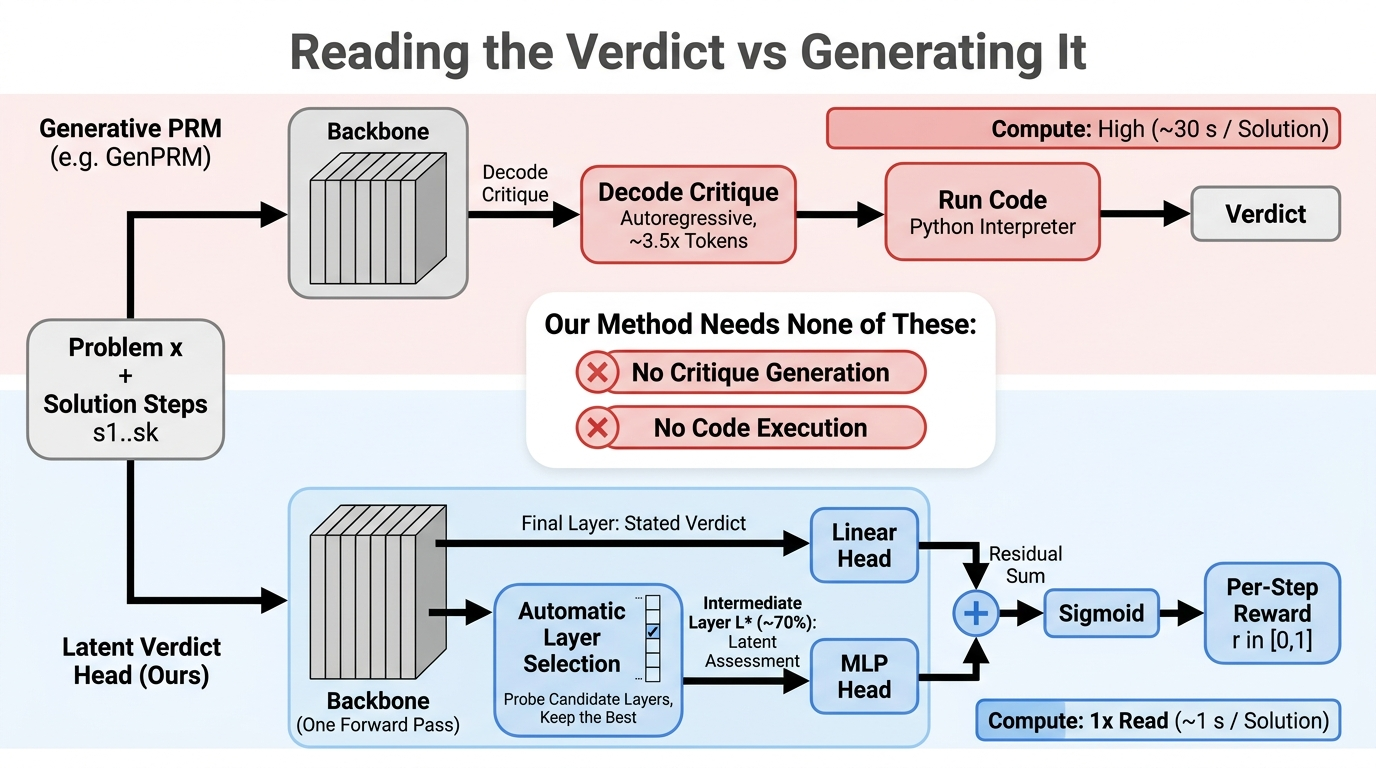
\includegraphics[width=0.9\linewidth]{figures/method_arch}}
    {\fbox{\parbox[c][4.2cm][c]{0.9\linewidth}{\centering\itshape figures/method\_arch.png \\ (architecture diagram: backbone with a mid layer and final layer tap, an MLP head and a linear head summed into a per step reward, one forward pass)}}}
  \caption{Reading the verdict instead of generating it. Top: a generative process reward model decodes a natural language critique, runs code, and often votes over several samples before a verdict, which costs many decoded tokens and an interpreter call. Bottom: the introspective verdict head reads the same solution in a single forward pass, taps the final layer for the stated verdict and an intermediate layer $\ell^\star$ for the latent assessment, and sums them into a per step reward. It needs no critique generation and no code execution, at about one quarter of the token cost of a single generative pass. Both methods use the same backbone and differ only in what follows it, and the intermediate layer $\ell^\star$ is selected automatically by a probe over candidate layers (\Cref{alg:select}).}
  \label{fig:arch}
\end{figure}

\subsection{Why an intermediate layer}
\label{sec:method-layer}

We place $\ell^\star$ at about seventy percent of the depth, nine layers below the output, which a per layer probe sweep selects (\Cref{fig:layersweep}). The reason is structural. The final state is optimized to emit the surface verdict token, so it is shaped by the form of the answer and can be moved by a step that reads fluently while being wrong. A state a few layers earlier is formed before that token is produced, and it aligns more closely with whether the step follows from its premises. The final layer corresponds to what the model would state, and the intermediate layer to the assessment that is present before the statement. \Cref{sec:exp-layer} shows that step correctness is in fact most separable at this depth and weaker at the final layer.

\subsection{Automatic layer selection}
\label{sec:method-select}

We do not fix $\ell^\star$ by hand. Before training, a cheap probe selects it automatically from a small labeled set, as in \Cref{alg:select}. For each candidate layer in a set $\cC$ we take the last token hidden state of every step, fit a class balanced logistic probe on step correctness, and score the located first error on a held out split. We set $\ell^\star$ to the candidate with the highest localization F1. The procedure runs once, passes no gradient through the backbone, and reuses the same step labels as training, so it adds little cost. It reads only the backbone's own features. The candidate set $\cC$ is fixed to the eight layers one, three, five, and so on up to fifteen below the output, and the labeled set is a few hundred solutions from the training distribution. We run the selection on the 7B backbone (\Cref{sec:exp-layer}), where it returns the layer nine below the output, near seventy percent of the depth, and since both backbones have 28 layers we apply the same relative depth $\ell^\star=20$ of $28$ at 1.5B. The training below then adapts the head at the selected $\ell^\star$.

\begin{algorithm}[t]
  \caption{Automatic selection of the intermediate layer $\ell^\star$}
  \label{alg:select}
  \begin{algorithmic}[1]
    \REQUIRE candidate layers $\cC$, labeled set $\cD_{\mathrm{sel}}$ with per step labels, split into fit and held out parts, frozen backbone $f$
    \FOR{each candidate layer $\ell \in \cC$}
      \STATE $X_\ell \leftarrow$ last token hidden states at layer $\ell$ for all steps in the fit part
      \STATE fit a class balanced logistic probe $p_\ell$ on $(X_\ell, y)$
      \STATE $F_\ell \leftarrow$ localization F1 of $p_\ell$ on the held out part
    \ENDFOR
    \RETURN $\ell^\star = \argmax_{\ell \in \cC} F_\ell$
  \end{algorithmic}
\end{algorithm}

\subsection{Training}
\label{sec:method-train}

We adapt the backbone with LoRA \citep{hu2021lora} of rank $16$ and scaling $32$ on the query, key, value, and output projections, and train the LoRA parameters and the two heads jointly. The rest of the backbone is frozen, and gradient checkpointing keeps the backbone and the heads within a single V100 class device at both the 1.5B and the 7B scale. Supervision is a set of step level labels $\cD=\{(x, s_{1:k}, y_{1:k})\}$ with $y_i\in\{0,1\}$, where $y_i=1$ marks an incorrect step. We minimize a class balanced binary cross entropy on the step logits of \Cref{eq:head},
\begin{equation}
  \cL \;=\; \sum_{(x,s_{1:k},y_{1:k})\in\cD}\ \sum_{i=1}^{k}\ \mathrm{BCE}\big(z_i,\, y_i\big),
  \qquad
  \text{positive weight } \frac{1-p}{p},
  \label{eq:loss}
\end{equation}
where $p$ is the fraction of error steps in $\cD$, which offsets the imbalance of rare errors. The labels come from the step level annotations released with GenPRM \citep{zhao2025genprm}. The method uses only these labels, not the generative model that produced them.

\begin{algorithm}[t]
  \caption{Introspective scoring of a $k$ step solution (inference)}
  \label{alg:score}
  \begin{algorithmic}[1]
    \REQUIRE problem $x$, steps $s_1,\dots,s_k$, adapted backbone $f$, heads $\vw, g$, layer $\ell^\star$, threshold $\tau$
    \STATE tokenize $x, s_1, \dots, s_k$ and record the last token index $t_i$ of each step
    \STATE $H \leftarrow f(x, s_{1:k})$ \hfill // one forward pass, hidden states at all layers, no decoding
    \FOR{$i = 1$ to $k$}
      \STATE $z_i \leftarrow \vw^\top H^{(L)}_{t_i} + g\big(H^{(\ell^\star)}_{t_i}\big)$; \quad $r_i \leftarrow \sigma(z_i)$
    \ENDFOR
    \STATE $e \leftarrow \min\{\, i : r_i > \tau \,\}$, or none if no step exceeds $\tau$
    \RETURN rewards $r_{1:k}$ and located first error $e$
  \end{algorithmic}
\end{algorithm}

\subsection{Inference and cost}
\label{sec:method-infer}

Inference is one forward pass. Given the problem and its steps we run the backbone once with hidden states, gather the last token index of each step, and apply \Cref{eq:head} to obtain $r_1,\dots,r_k$, as in \Cref{alg:score}. The located first error is the first step whose reward exceeds a threshold $\tau$, and $\tau$ is fixed on a held out split. There is no autoregressive decoding and no interpreter call. The cost is a single prefill over the solution of $n$ tokens, against a generative verifier that prefills the same solution and then decodes a critique on the order of $c\,n$ tokens and runs code, one forward pass per generated token. A solution with $k$ steps is therefore scored at the cost of reading it once, and \Cref{sec:exp-compute} quantifies the gap.

\subsection{Fusion with a generative verifier}
\label{sec:method-fusion}

The introspective reward and a generative verifier read different evidence, so they can be combined. Given a generative verifier's per step correctness probability $P^{B}_i$, we form a logit space score
\begin{equation}
  \zeta_i \;=\; a\,\big(z_i - c\big) \;+\; (1-a)\,\mathrm{logit}\big(1 - P^{B}_i\big),
  \label{eq:fusion}
\end{equation}
and locate the first error at the first step with $\zeta_i$ above a bias $b$. The weight $a$ and bias $b$ are fixed on a held out split and never tuned on the evaluated subset, which keeps the combination honest. The scalar $c$ is an unsupervised per domain centering that we apply only at the 7B scale, and we explain in \Cref{app:calib} why the 7B head needs it and the 1.5B head does not. The fusion adds one forward pass to the generative pipeline, so it is close to free next to repeated decoding.
